\section*{Introduction}
Dans ce chapitre, nous présenterons le jeu de données, les analyses audio-MIDI.\\
Nous ferons la démonstration d’un modèle théorique de système (implémentable) qui devra être utilisé comme base de connaissances pour obtenir un système plus rapide et une meilleure qualité en sortie.\\
Enfin, nous présenterons les différentes contributions de développement.
\section{Le jeu de données}
Nous avons utilisé le Groove MIDI Dataset\footnote{\url{https://magenta.tensorflow.org/datasets/groove}} \cite{groove2019} (GMD) qui est un jeu de donnée mis à disposition par Google sous la licence Creative Commons Attribution 4.0 International (CC BY 4.0).\\
Le GMD est composé de 13,6 heures de batterie sous forme de fichiers MIDI et audio alignés. Il contient 1150 fichiers MIDI et plus de 22 000 mesures de batterie dans les styles les plus courants et avec différentes qualités de jeu. Tout le contenu a été joué par des humains sur la batterie électronique Roland TD-11 (figure \ref{electro_drums}).\newpage
\begin{figure}[h]
	\centering
	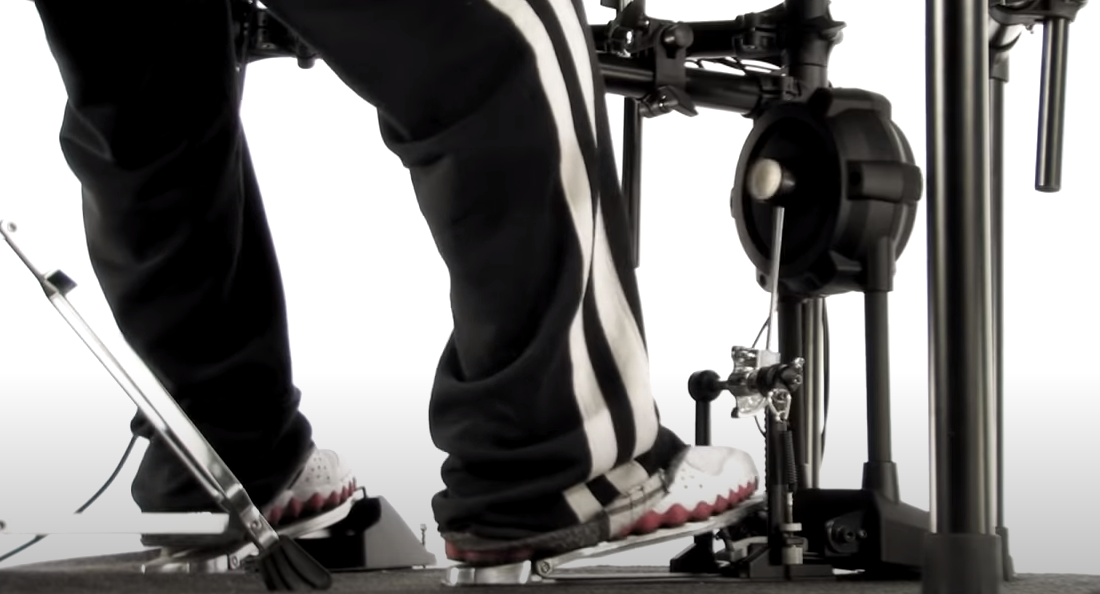
\includegraphics[height=35mm, width=60mm]{z_images/4_experimentations/0_groove/0_roland.png}\ \ 
	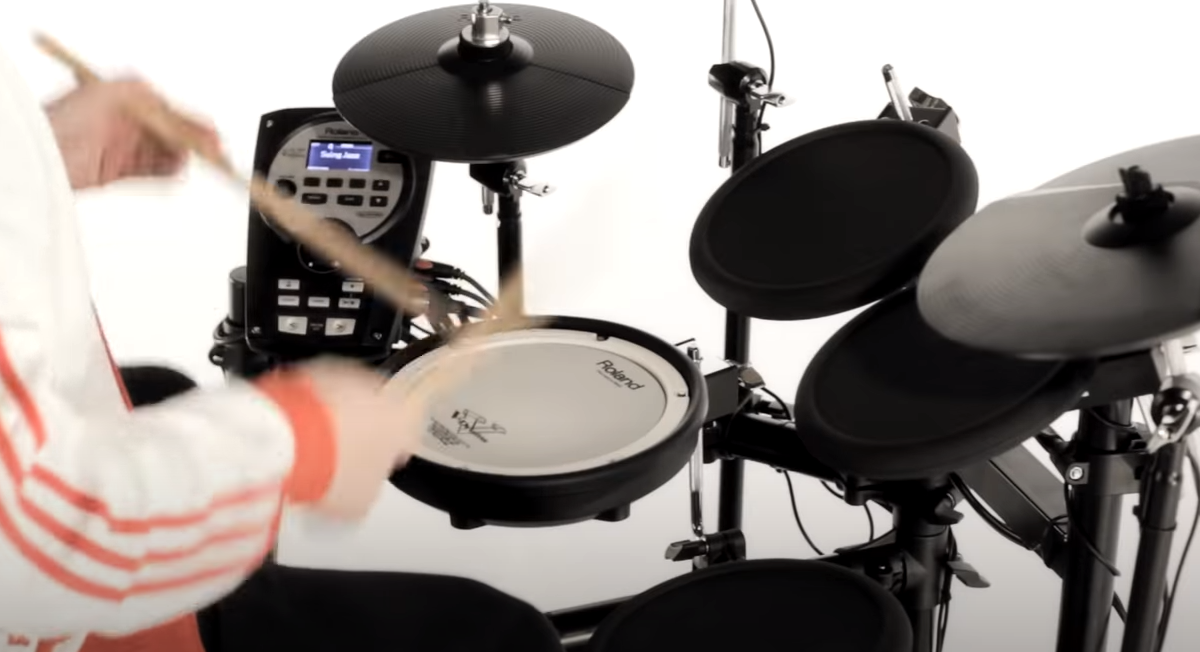
\includegraphics[height=35mm, width=60mm]{z_images/4_experimentations/0_groove/1_roland.png}
	\caption{Batterie électronique}
	\label{electro_drums}
	\textit{Source :} \url{https://www.youtube.com/watch?v=BX1V_IE0g2c}
\end{figure}
Autres critères spécifiques au GMD :
\begin{itemize}
	\item Toutes les performances ont été jouées au métronome et à un tempo choisi par le batteur.
	\item 80\% de la durée du GMD a été joué par des batteurs professionnels qui ont pu improviser dans un large éventail de styles. Les données sont donc diversifiées en terme de styles et de qualités de jeu (professionnel ou amateur).
	\item Les batteurs avaient pour instruction de jouer des séquences de plusieurs minutes ainsi que des fills\footnote{Un \textit{fill} est une séquence de relance dont la durée dépasse rarement 2 mesures. Il est souvent joué à la fin d’un cycle pour annoncer le suivant.}
	\item Chaque performance est annotée d’un style (fourni par le batteur), d’une métrique et d’un tempo ainsi que d’une identification anonyme du batteur.
	\item Il a été demandé à 4 batteurs d’enregistrer le même groupe de 10 rythmes dans leur style respectifs. Ils sont dans les dossiers eval-session du GMD.
	\item Les sorties audio synthétisées ont été alignées à 2 ms près sur leur fichier MIDI.
\end{itemize}
\subsection*{Format des données}
Le Roland TD-11 divise les données enregistrées en plusieurs pistes distinctes :
\begin{itemize}
	\item une pour le tempo et l’indication de mesure ;
	\item une pour les changements de contrôle (position de la pédale de charley) ;
	\item une pour les notes.\\
\end{itemize}
Les changements de contrôle sont placé sur le canal 0 et les notes sur le canal 9 (qui est le canal canonique pour la batterie).\\
Pour simplifier le traitement de ces données, ces trois pistes ont été fusionnées en une seule piste qui a été mise sur le canal 9.\\\\
« Control Changes
The TD-11 also records control changes specifying the position of the hi-hat pedal on each hit. We have preserved this information under control 4. »\\(\url{https://magenta.tensorflow.org/datasets/groove})\\$\Rightarrow$ ??? Je ne comprends pas encore comment trouver ce type d’informations dans les fichiers MIDI.\\L’utilisation de pretty\_midi devient urgente !
\section{Analyse MIDI-Audio}
\label{analyse_midi_audio}
Ces analyses ont été faites dans le cadre de transcriptions manuelles à partir de fichiers MIDI et Audio du GMD. Les transcriptions manuelles ont été éditées à l’aide de lilypond\footnote{\url{http://lilypond.org/}}. Les transcriptions automatiques ont été générées manuellement avec MuseScore\footnote{\url{https://musescore.com/}}.
\subsection*{Comparaisons de transcriptions}
\subsubsection{drummer\_01/session3}
\tab \tab \tab \tab Transcription manuelle $\Rightarrow$ Transcription musescore
\begin{figure}[h]
	\centering
	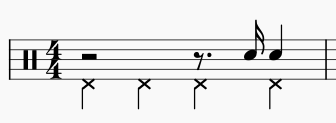
\includegraphics[height=20mm, width=50mm]{z_images/4_experimentations/1_analyse_midi_audio/0_drummer1_session3/1_manuelle.png}\ \ \ \ 
	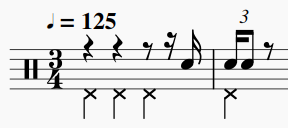
\includegraphics[height=20mm, width=45mm]{z_images/4_experimentations/1_analyse_midi_audio/0_drummer1_session3/0_musescore.png}
	\caption{Exemple d’analyse 1}
\end{figure}
\begin{itemize}
	\item Erreur d’indication de mesure (3/4 au lieu de 4/4) ;
	\item Les silences de la premiere mesure sont inutilement surchargés ;
	\item La noire du quatrième temps de la première mesure est devenue les deux première notes (une double-croche et une croche) d’un triolet sur le premier temps de la deuxième mesure.\\
\end{itemize}\newpage
\tab \tab \tab \tab Transcription manuelle $\Rightarrow$ Transcription musescore
\begin{figure}[h]
	\centering
	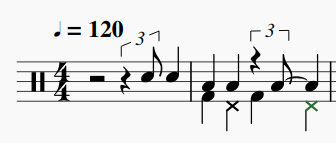
\includegraphics[height=25mm, width=60mm]{z_images/4_experimentations/1_analyse_midi_audio/0_drummer1_session3/3_manuelle.png}\ \ \ \ 
	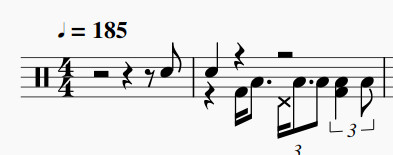
\includegraphics[height=25mm, width=55mm]{z_images/4_experimentations/1_analyse_midi_audio/0_drummer1_session3/2_musescore.png}
	\caption{Exemple d’analyse 2}
\end{figure}\\
\begin{itemize}
	\item L’indication de mesure est correcte mais tout a été décalé d’un temps car la première noire sur la caisse claire est jouée sur le 4ème temps et non sur le premier temps de la deuxième mesure comme l’indique la transcription de musescore.
	\item Les toms basses des 1er et 2ème temps de la mesure musescore auraient dû être sur les temps et non décalés d’une double croche vers la droite.\\
\end{itemize}
\tab \tab \tab \tab Transcription manuelle $\Rightarrow$ Transcription musescore
\begin{figure}[h]
	\centering
	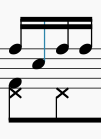
\includegraphics[height=20mm, width=15mm]{z_images/4_experimentations/1_analyse_midi_audio/0_drummer1_session3/5_manuelle.png}\ \ \ \ 
	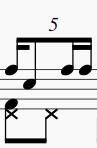
\includegraphics[height=20mm, width=15mm]{z_images/4_experimentations/1_analyse_midi_audio/0_drummer1_session3/4_musescore.png}
	\caption{Exemple d’analyse 3}
\end{figure}
\begin{itemize}
	\item Erreur de quantification : les doubles croches ont été interprétées en quintolet;\\
\end{itemize}
\subsubsection{drummer\_01/session1}
\tab \tab \tab \tab Transcription manuelle $\Rightarrow$ Transcription musescore
\begin{figure}[h]
	\centering
	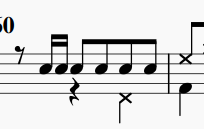
\includegraphics[height=25mm, width=40mm]{z_images/4_experimentations/1_analyse_midi_audio/1_drummer1_session1/1_manuelle.png}\ \ \ \ 
	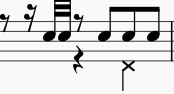
\includegraphics[height=25mm, width=40mm]{z_images/4_experimentations/1_analyse_midi_audio/1_drummer1_session1/0_musescore.png}
	\caption{Exemple d’analyse 4}
\end{figure}
\begin{itemize}
	\item On dirait que lorsque certaines notes sont proches, elles se resserrent et suppriment celles qui aurait dû être sur le temps.\\
\end{itemize}
\tab \tab \tab \tab Transcription manuelle $\Rightarrow$ Transcription musescore
\begin{figure}[h]
	\centering
	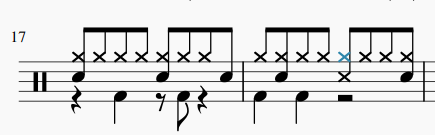
\includegraphics[height=20mm, width=50mm]{z_images/4_experimentations/1_analyse_midi_audio/1_drummer1_session1/3_manuelle.png}\ \ \ \ 
	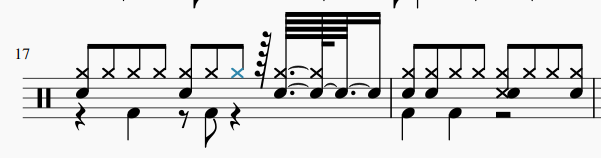
\includegraphics[height=20mm, width=70mm]{z_images/4_experimentations/1_analyse_midi_audio/1_drummer1_session1/2_musescore.png}
	\caption{Exemple d’analyse 5}
\end{figure}
Le 2ème croche du 4ème temps !!
\subsubsection{Exemple avec des flas}
Transcription avec musescore :\\
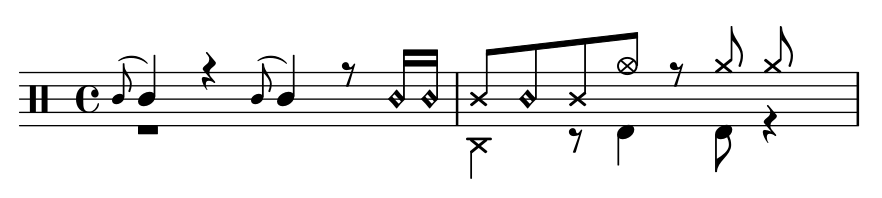
\includegraphics[height=30mm, width=120mm]{z_images/4_experimentations/1_analyse_midi_audio/2_transcriptions_flas/0_124_funk_95_fill_4-4.png}\\
Transcription manuelle :\\
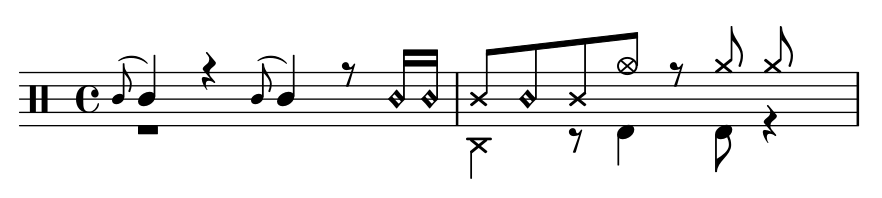
\includegraphics[height=20mm, width=90mm]{z_images/4_experimentations/1_analyse_midi_audio/2_transcriptions_flas/1_124_funk_95_fill_4-4.png}\\
MuseScore donne un aperçu de l’état de l’art pour la transcription de la batterie.
\newpage
\subsection*{Transcription de partition}
\begin{figure}[h]
	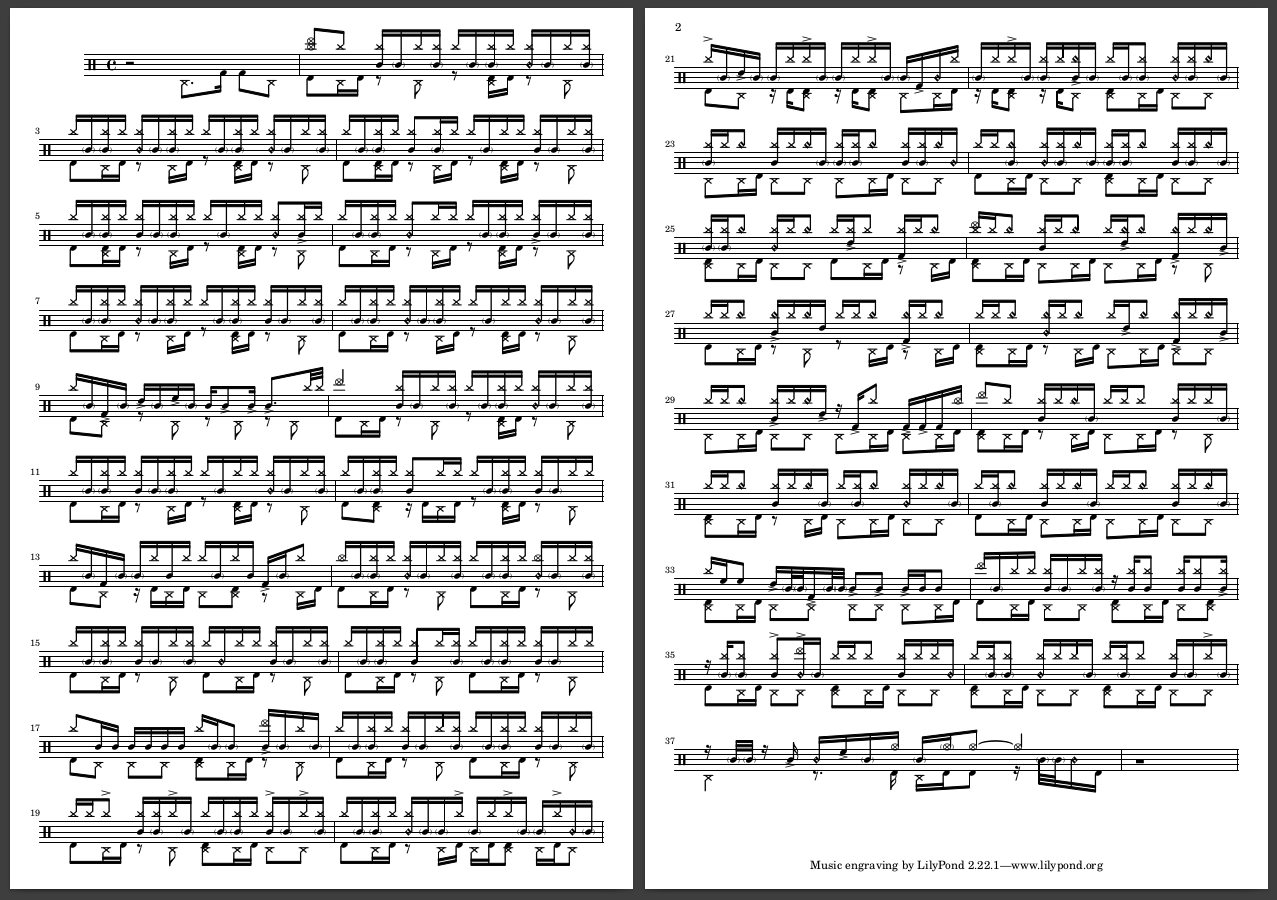
\includegraphics[height=120mm, width=160mm]{z_images/4_experimentations/1_analyse_midi_audio/3_partition.png}
	\caption{Partition entière}
	\label{partition_entiere}
\end{figure}
Il s’agit d’une partition d’un 4/4 binaire dont le fichier MIDI est annoncé dans le groove-dataset de style «jazz-funk» probablement en raison de la ride de type shabada rapide (le ternaire devient binaire avec la vitesse) combiné avec l’after-beat de type rock (caisse-claire sur les deux et quatre).\\
La transcription de cette partition a occasionné plusieurs remarque :\\
- vélocité, place des accents, etc…
\section{Expérimentation théorique d’un système}
\subsection*{Motifs}
\begin{figure}[h]
	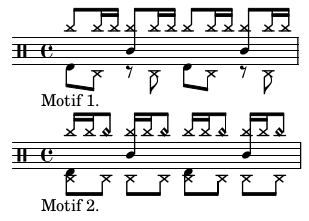
\includegraphics[height=30mm, width=40mm]{z_images/4_experimentations/2_demonstration_systeme/0_motifs_4-4_binaires.png}
	\caption{Motifs}
\end{figure}
Les motifs 1 et 2 peuvent être extraits de la figure 3.8. Ces deux motifs sont très classiques et seront réutilisables aussi dans d’autres contextes.\\
Le motif 1 est joué jusqu’à la mesure 18 avec des variations et des breaks.\\
Le motif 2 est joué des mesures 23 à 28.\\\\
\subsection*{Gammes}
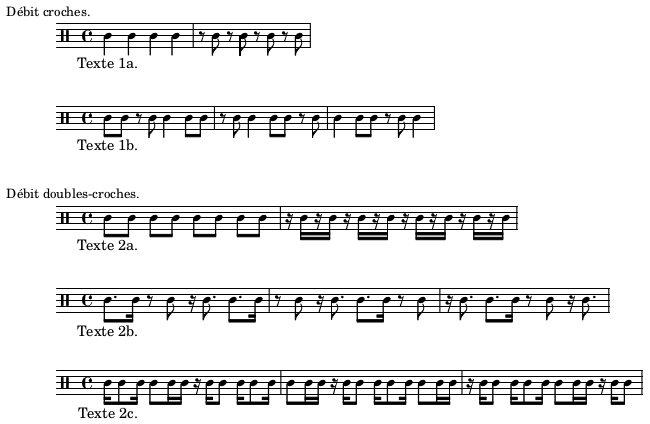
\includegraphics[height=70mm, width=95mm]{z_images/4_experimentations/2_demonstration_systeme/1_gammes_4-4_binaires.png}\\

\subsection*{Systèmes}
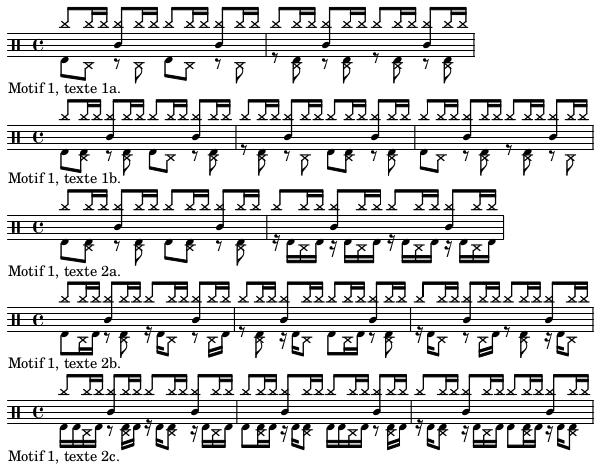
\includegraphics[height=75mm, width=85mm]{z_images/4_experimentations/2_demonstration_systeme/2_systeme_4-4_binaire.png}
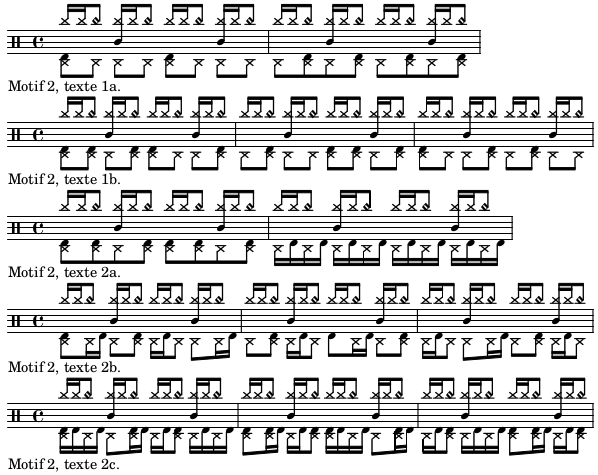
\includegraphics[height=75mm, width=85mm]{z_images/4_experimentations/2_demonstration_systeme/3_systeme_4-4_binaire.png}
\newpage

\subsection*{Démonstration}
\label{demo_sys}
\textbf{Représentation des systèmes en arbres de rythmes}

\resizebox{440pt}{!} {
	\Tree[.Motif\ 1\ +\ Texte\ 1a
	[.Mesure\ 1
	[.Temps\ 1 [rd\\bd ][ [rd\\pf ][rd ]]]
	[.Temps\ 2 [rd\\cc ][ [rd\\pf ][rd ]]]
	[.Temps\ 3 [rd\\bd ][ [rd\\pf ][rd ]]]
	[.Temps\ 4 [rd\\cc ][ [rd\\pf ][rd ]]] ]
	[.Mesure\ 2
	[.Temps\ 1 [rd ][ [rd\\bd\\pf ][rd ]]]
	[.Temps\ 2 [rd\\cc ][ [rd\\bd\\pf ][rd ]]]
	[.Temps\ 3 [rd ][ [rd\\bd\\pf ][rd ]]]
	[.Temps\ 4 [rd\\cc ][ [rd\\bd\\pf ][rd ]]] ]]}
\textbf{Réécriture}
\textit{Règles établies par le système}\\
\textbf{Séparation des voix}\\
\\\\
Ainsi l’arbre syntaxique de départ sera divisé en autant d’instruments qui le constituent et les voix seront regroupées de manière cohérentes.
\textit{Voix haute}\\
\resizebox{440pt}{!} {
	\Tree[.Motif\ 1\ +\ Texte\ 1a
	[.Mesure\ 1
	[.Temps\ 1 [rd ][ [rd ][rd ]]]
	[.Temps\ 2 [rd\\cc ][ [rd ][rd ]]]
	[.Temps\ 3 [rd ][ [rd ][rd ]]]
	[.Temps\ 4 [rd\\cc ][ [rd ][rd ]]] ]
	[.Mesure\ 2
	[.Temps\ 1 [rd ][ [rd ][rd ]]]
	[.Temps\ 2 [rd\\cc ][ [rd ][rd ]]]
	[.Temps\ 3 [rd ][ [rd ][rd ]]]
	[.Temps\ 4 [rd\\cc ][ [rd ][rd ]]] ]]}\\

\textit{Voix basse}\\
\resizebox{440pt}{!} {
	\Tree[.Motif\ 1\ +\ Texte\ 1a
	[.Mesure\ 1
	[.Temps\ 1 [bd ][ [pf ][t ]]]
	[.Temps\ 2 [t ][ [pf ][t ]]]
	[.Temps\ 3 [bd ][ [pf ][t ]]]
	[.Temps\ 4 [t ][ [pf ][t ]]] ]
	[.Mesure\ 2
	[.Temps\ 1 [t ][ [bd\\pf ][t ]]]
	[.Temps\ 2 [t ][ [bd\\pf ][t ]]]
	[.Temps\ 3 [t ][ [bd\\pf ][t ]]]
	[.Temps\ 4 [t ][ [bd\\pf ][t ]]] ]]}\\

\textbf{Règles de simplifications pour le 4/4 binaire}\\
Simplifier l’écriture de chaque voix (\textit{Règles établis par le système})\\
\resizebox{70pt}{!} {
	\Tree[.1/4 [t ][x ][x ][x ] ]
}\ \ \ \ \ $\Rightarrow$\ \ \ \ \
\resizebox{70pt}{!} {
	\Tree[.1/4 [r ][x ][x ][x ] ]
}\\\\

\resizebox{70pt}{!} {
	\Tree[.1/4 [x ][t ][x ][x ]]
}\ \ \ \ \ $\Rightarrow$\ \ \ \ \
\resizebox{50pt}{!} {
	\Tree[.1/4 [x ][ [x ][x ]]]
}\\\\

\resizebox{70pt}{!} {
	\Tree[.1/4 [t ][x ][x ][t ] ]
}\ \ \ \ \ $\Rightarrow$\ \ \ \ \
\resizebox{50pt}{!} {
	\Tree[.1/4 [ [r ][x ]][x ] ]
}\\\\

\resizebox{50pt}{!} {
	\Tree[.1/4 [t ][ [x ][x ]]]
}\ \ \ \ \ $\Rightarrow$\ \ \ \ \
\resizebox{50pt}{!} {
	\Tree[.1/4 [r ][ [x ][x ]]]
}\\\\

\resizebox{50pt}{!} {
	\Tree[.1/4 [t ][ [x ][t ]] ]
}\ \ \ \ \ $\Rightarrow$\ \ \ \ \
\resizebox{30pt}{!} {
	\Tree[.1/4 [r ][x ] ]
}\\\\

\resizebox{50pt}{!} {
	\Tree[.1/4 [x ][ [x ][t ]] ]
}\ \ \ \ \ $\Rightarrow$\ \ \ \ \
\resizebox{30pt}{!} {
	\Tree[.1/4 [x ][x ] ]
}
\section{Développement}
\subsection*{DrumCode}
Adaptation de la modélisation pour la transcription en cpp.
\subsection*{Tests unitaires sur les Jams}
\label{jam_tests}
Les Jams permettent de passer du monophonique au polyphonique.
\subsection*{Parsing}
\label{gram_pond}
Tests effectués avec le fichier midi suivant :\\\\
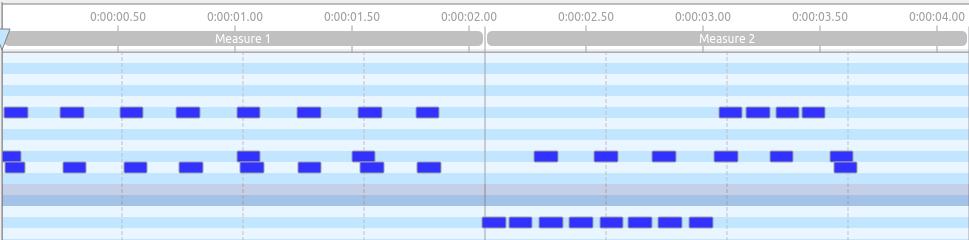
\includegraphics[height=50mm, width=160mm]{z_images/4_experimentations/3_developpement/0_midi_2bars_fill.png}\\\\
%\textit{Voix basse}\\
Un premier test convaincant est effectué avec la grammaire suivante :\\\\
// bar level\\
0 -> C0                1\\
0 -> E1                1\\
0 -> U4(1, 1, 1, 1)    1\\

// half bar level\\
9 -> C0                1\\
9 -> E1                1\\

// beat level\\
1 -> C0                1\\
1 -> E1                1\\
1 -> T2(2, 2)          1\\
1 -> T4(4, 4, 4, 4)    1\\

// croche level\\
2 -> C0                1\\
2 -> E1                1\\

// double level\\
4 -> C0                1\\
4 -> E1                1\\
4 -> E2                1\\
4 -> T2(6, 6)          1\\

// triple level\\
6 -> E1                1\\\\
Cette grammaire sépare les ligatures par temps au niveau de la mesure. Puis, au niveau du temps, elle autorise les divisions par deux (croches) et par quatre (doubles-croches). Tous les poids sont réglés sur 1. L’arbre de parsing en résultant est considéré comme « convaincant » car il découpe correctement les mesures et les temps.
\\\\
\resizebox{450pt}{!} {
\Tree[.Mesure\ 1
[.Temps\ 1 [0-ON\\1-ON\\2-ON ][3-OFF\\4-OFF\\5-OFF ][6-ON\\7-ON ][8-OFF\\9-OFF ]]
[.Temps\ 2 [10-ON\\11-ON ][12-OFF\\13-OFF ][14-ON\\15-ON ][16-OFF\\17-OFF ]]
[.Temps\ 3 [18-ON\\19-ON\\20-ON ][21-OFF\\22-OFF\\23-OFF ][24-ON\\25-ON ][26-OFF\\27-OFF ]]
[.Temps\ 4 [28-ON\\29-ON\\30-ON ][31-OFF\\32-OFF\\33-OFF ][34-ON\\35-ON ][36-OFF\\37-OFF ]]
]}\\\\\\
Les temps de la première mesure du fichier MIDI sont bien quantifié mais ceux de la deuxième mesure présentent quelques défauts de quantification visibles dès le premier temps.\\\\
\resizebox{300pt}{!} {
\Tree[.Mesure\ 2
[.Temps\ 1 [38-ON ][ [39-OFF ][40-ON ] ][ [41-OFF\\42-ON ][43-ON ] ][ [44-OFF\\45-OFF ][46-ON ] ]]
]}\\\\\\
Les Onsets sont correctement triés au niveau des doubles croches mais certaines doubles croches sont inutilement subdivisées en triples croches (les 2ème, 3ème et 4ème doubles croches sur le premier temps ci-dessus).\\\\
\textbf{2ème exemple :}\\
Après une augmentation du poids des triples croches dans la grammaire (monté de 1 à 5)et une baisse de tous les autres poids (descendu de 1 à 0.5), et mis à part le troisième temps de la 2ème mesure, tous les Onsets sont bien triés et aucuns ne sont subdivisés.






%\newpage
%\section{Résultats et discussion}
%\subsection{Résultats}
%\subsection{Évaluation}
%1 - Transcription manuelle à partir de fichier midi et/ou wav d’une partition contenant des systèmes. Écriture des systèmes contenues dans la partition (arbres, séparation des voix, réécriture)\\\\

\section*{Conclusion}
Conclusion de ce chapitre.